\chapter{Background}

    \section{Introduction}

    \section{Bluetooth Low Energy}
      \subsection{Scanning and Advertising}
      The Packet data unit for the advertising channel (called the Advertising
      Channel PDU) includes a 2-byte header and a variable payload from 6 to 37
      bytes. The actual length of the payload is defined by the 6-bit Length field
      in the header of the Advertising Channel PDU.

      there are several PDU types for the advertisements, but here we will focus
      ADV\_NONCONN\_IND - peripheral does not want to accept connections, which is
      typical in Beacons.

      \FloatBarrier
      \begin{figure}[h]
        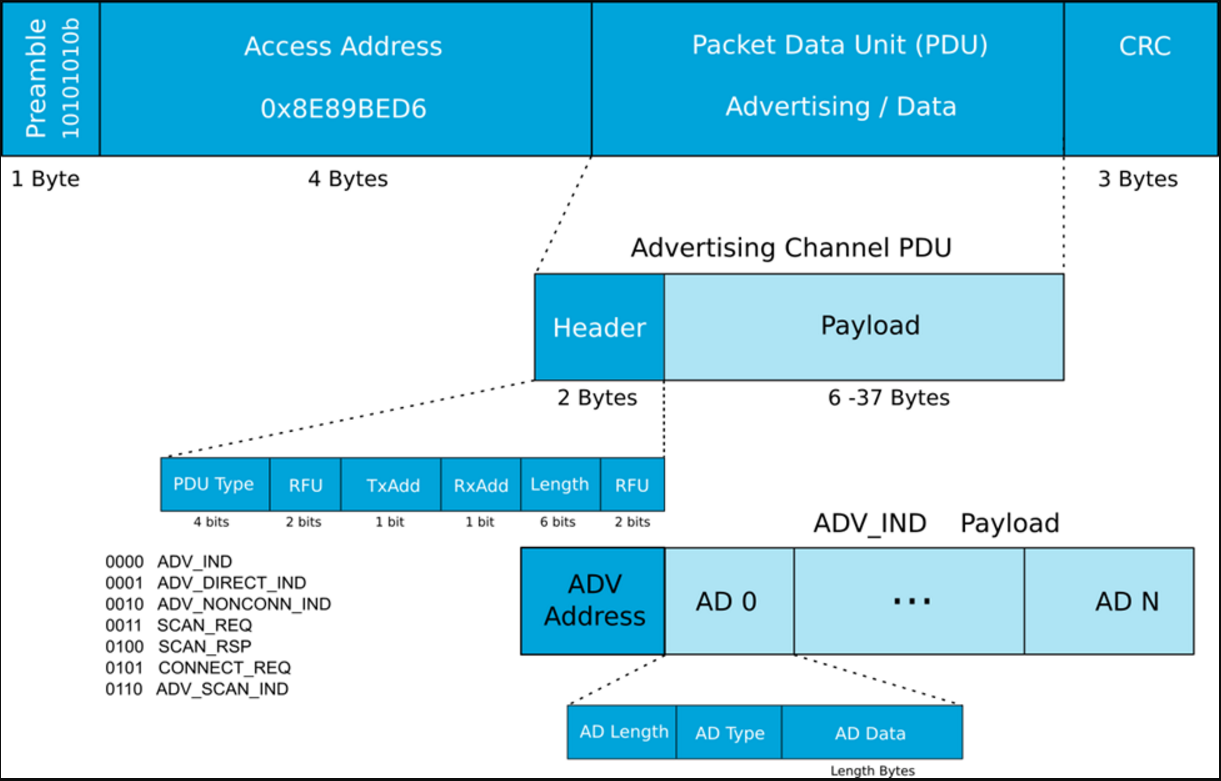
\includegraphics[width=\textwidth]{Images/ble_advertisement_packet.PNG}
      \end{figure}
      \FloatBarrier

      \FloatBarrier
      \begin{figure}[h]
        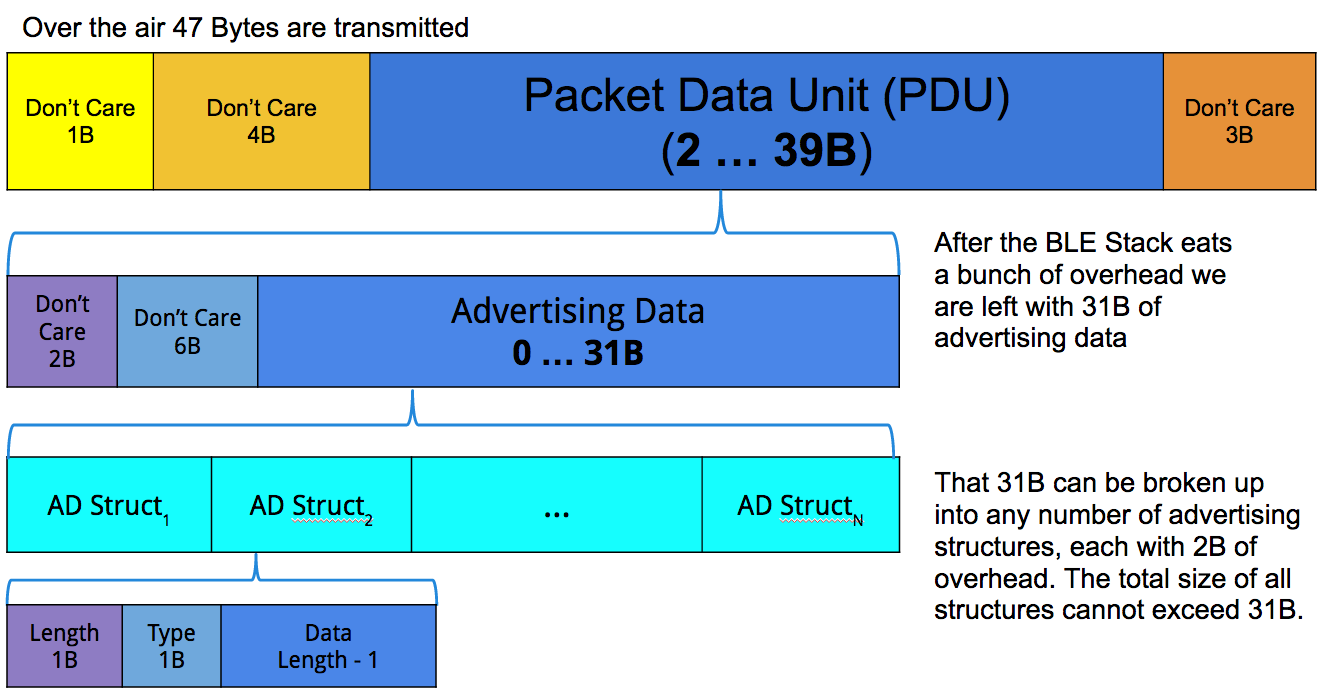
\includegraphics[width=\textwidth]{Images/general_structure.png}
      \end{figure}
      \FloatBarrier

      \FloatBarrier
      \begin{figure}[h]
        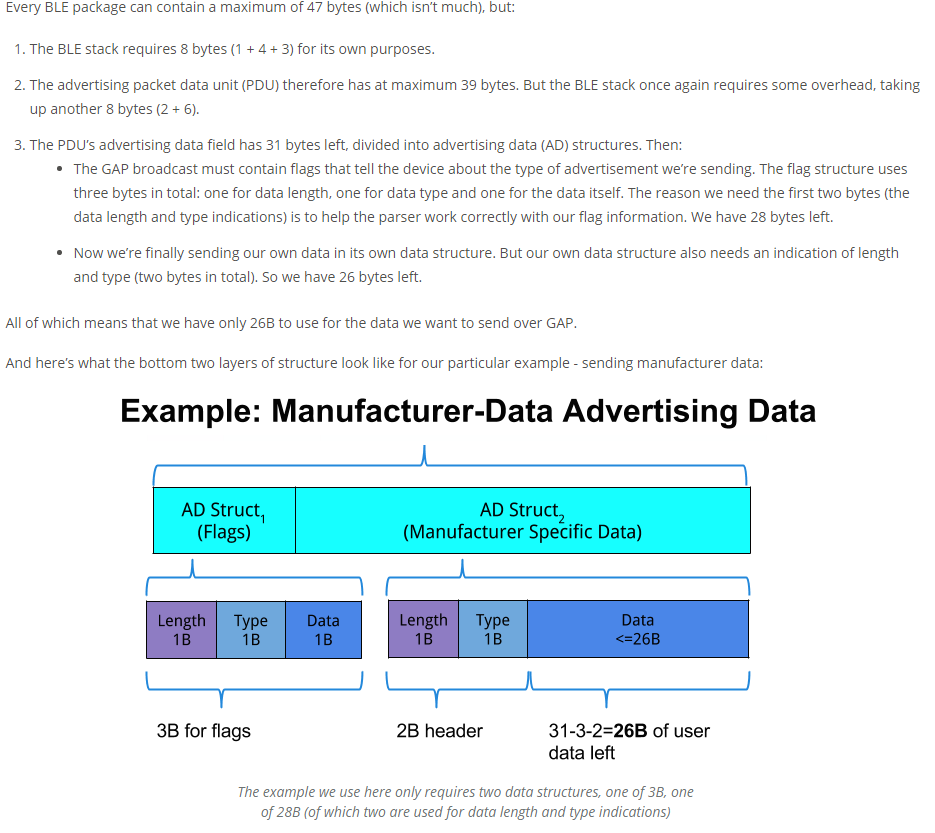
\includegraphics[width=\textwidth]{Images/packet_example.png}
      \end{figure}
      \FloatBarrier
      http://www.argenox.com/a-ble-advertising-primer/

      https://docs.mbed.com/docs/ble-intros/en/latest/Advanced/CustomGAP/

    \section{Investigated Protocols}
      \subsection{AODV}
      \subsubsection{Overview}
      AODV is a reactive routing protocol designed for use in ad hoc networks.
      Ad hoc networks are networks which have no pre-existing infrastructure and
      so AODV is particularly suitable for peer-to-peer BLE networks. In AODV,
      topology information is only transmitted on demand. Only a single route is
      ever recorded between a source and destination, and is only maintained while
      active. An example of this protocol can be seen in figure 1.

      When a node wishes to send traffic to a host and no route is known, a route
      request (RREQ) message is broadcast. At each node the RREQ arrives at, if
      the node is not the destination and does not have a route recorded, it
      rebroadcasts the RREQ. A route is considered found when the RREQ message
      arrives at either the desired host, or to an intermediary node with a valid
      route entry for the destination. In either case, a route reply message (RREP)
      is sent back to the originator of the RREQ message. As the RREP message
      propagates back to the originator, each intermediary node creates a route
      to the destination.

      Hello messages can be used to detect link breaks. Nodes periodically
      broadcast these Hello messages to their neighbours and in the event that a
      node fails to receive several Hello message from its neighbour, a break is
      detected. In the event that a node detects an error in one of its known
      routes, it sends a route error (RERR) message to each of its neighbours.

      The AODV protocol has built in sequencing numbers in each RREQ and RREP
      packet which prevents routing loops being formed, a challenge faced by many
      routing algorithms. In addition to this, each node maintains its own routing
      table, keeping the routing process minimal if the host has the required
      route information in its own routing table.

      C. E. Perkins, E. M. Belding-Royer, and S. Das. "Ad hoc OnDemand Distance
      Vector (AODV) Routing" RFC 3561, July 2003.

      \subsubsection{Evaluation}

      \subsubsection{BLE Considerations}
      \FloatBarrier
      \begin{figure}[h]
        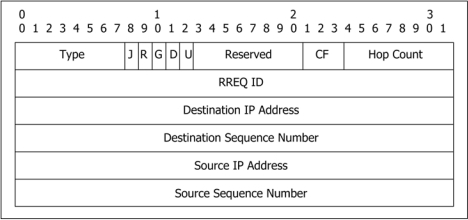
\includegraphics[width=\textwidth]{Images/rreq_packet_format.png}
      \end{figure}
      \FloatBarrier
      Total size: 24 Bytes

      \subsection{LOADng}
      T. Clausen et al. “The Lightweight On-demand Ad hoc Distance-vector Routing Protocol
- Next Generation (LOADng)”. In: Internet Engineering Task Force (IETF) Draft
(2016)

      \subsection{Trickle}
      P. Levis, T. Clausen, J. Hui, O. Gnawali, J. Ko, The Trickle Algorithm, IETF
      Internet Draft: draft-ietf-roll-trickle-08, 2011

      \subsection{LOAD}
      K. Kim, S. Daniel Park, G. Montenegro, S. Yoo, N. Kushalnagar,
6LoWPAN Ad Hoc On-Demand Distance Vector Routing (LOAD), IETF
Internet Draft: draft-daniel-6lowpan-load-adhoc-routing-03, 2007.

      \subsection{ZigBee Cluster Tree protocol}
      S.C. Erge, ZigBee/IEEE 802.15.4 Summary, 2004. <http://
staff.ustc.edu.cn/ustcsse/papers/SR10.ZigBee.pdf>.

      \subsection{Hilow}
      K. Kim, S. Yoo, J. Park, S.D. Park, J. Lee, Hierarchical Routing over
6LoWPAN (HiLow), IETF: Internet Draft: draft-deniel-6lowpanhilow-hierarchical-routing-00.txt,
vol. 38, December 2005.

      \subsection{Dymo-Low}
      K. Kim, S. Park, I. Chakeres, C. Perkins, Dynamic MANET On-demand
for 6LoWPAN (DYMO-low) Routing, Internet Draft: draftmontenegro-6lowpan-dymo-low-routing-03,
June 2007

      \subsection{RPL}
        \subsubsection{Overview}
        RPL is based on the topological concept of Directed Acyclic
        Graphs (DAGs). The DAG defines a tree-like structure
        that specifies the default routes between nodes in the
        LLN.

        RPL organizes nodes as Destination-Oriented DAGs (DODAGs), where most
        popular destination nodes (i.e. sinks) or those providing a
        default route to the Internet (i.e. gateways) act as the roots
        of the DAGs.

        A network may consist of one or several DODAGs, which form together an
        RPL instance identified by a unique ID, called RPLInstanceID.

        Olfa Gaddour, Anis Koubâa, "RPL in a nutshell: A survey", Computer Networks
Volume 56, Issue 14, 28 September 2012, Pages 3163–3178

        \FloatBarrier
        \begin{figure}[h]
          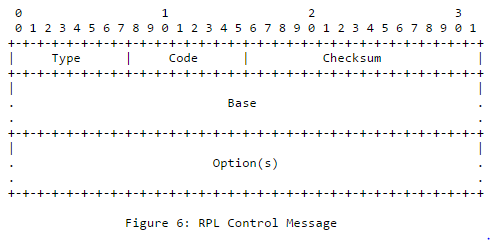
\includegraphics[width=\textwidth]{Images/rpl_control_packet_format.png}
        \end{figure}
        \FloatBarrier

        \subsubsection{Evaluation}
        Aishwarya Parasuram, "An Analysis of the RPL Routing Standard for Low Power
        and Lossy Networks", May 14, 2016

        \begin{itemize}
        \item
        RPL does not support applications which require a fixed MTU (Maximum Transmission
  Unit). The control message size can vary greatly and RPL does not give any
  guarantees on the size.

        \item
        RPL does not cater well to a request-response traffic pattern such as utility metering[24]

        Ulrich Herberg and Thomas Clausen. “A Comparative Performance Study of the Routing
        Protocols LOAD and RPL with Bi-Directional Trac
        in Low-power and Lossy Networks
        (LLN)”

        \item
        RPL does not cater to emergency scenarios where there is a high data trac in the
  network. In case of an emergency, a number of messages might be sent out causing
  congestion at the DODAG root. It also causes delay and possible packet loss [68].
  RPL doesn’t specify any mechanism of dealing with data packet loss.

      Weisheng Tang et al. “Toward Improved RPL: A Congestion Avoidance Multipath
  Routing Protocol with Time Factor for Wireless Sensor Networks”. In: Journal of
  Sensors 2016 (2015).

        \item
        RPL cannot be used for topologies with a long chain-like structure that contains paths
  length greater than eight (if raw IPv6 is used) or 64 (while using IPv6 address
  compression [31]), while being used in non-storing mode. The source routing header
  can be a maximum of 136 octets which includes an eight octet long header. An IPv6
  address is 16 octets long. Hence no more than eight can be accommodated unless
  address compression is used. If the addresses are compressed, then the path length
  may not exceed 64.

        Ed. J. Hui and P. Thubert. “Compression Format for IPv6 Datagrams over IEEE
  802.15.4-Based Networks”. In: Internet Engineering Task Force (IETF) 4944 (2011).

        \item
        In the current specification there is no support provided for broadcast. RPL only
  supports unicast to and from the DODAG root. In case broadcast is required, the root
  has to deliver the data to all nodes, which is very inecient.

        \item
        RPL is not suitable for WSNs that contain sensor nodes that can harvest ambient
  energy from the environment. Such networks are a possible solution for sustaining
  sensor networks for decades without maintenance, since they can recharge on their
  own using ambient energy. However in [47], it was found that energy-harvesting sensor
  networks running RPL produce 40-45\% lower goodput than battery-operated sensor
  networks as the harvesters drop

        Wilbert Nestor Michael C. Tiglao, China Kimberly Paige S. Yu, and Carl C. Dizon.
  “Performance Analysis of RPL in an Ambient Energy Harvesting Wireless Sensor Network”.
  In: The 4th International Conference on Internet Applications, Protocols and
  Services (NETAPPS) (2015).
  \end{itemize}
    \section{Summary}
